% \documentclass{book}
% \usepackage{tikz, libertine, ifthen}
% \begin{document}
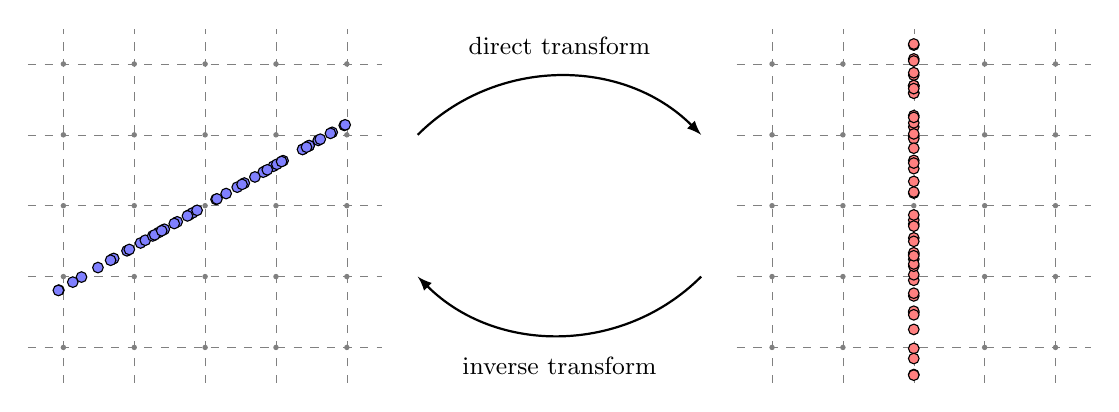
\begin{tikzpicture}[scale=0.9]
\tikzstyle{every node}=[font=\small]

	\draw[style=help lines, dashed, very thin, rotate=0] (0.5,0.5) grid (5.5,5.5);
	\draw[style=help lines, dashed, very thin, rotate=0] (10.5,0.5) grid (15.5,5.5);

	\foreach \x in {1,2,...,5} {
		\foreach \y in {1,2,...,5} {
			\filldraw [black!50, opacity = 1] (\x,\y) circle (0.03);
		}
	}

	\foreach \x in {11,12,...,15} {
		\foreach \y in {1,2,...,5} {
			\filldraw [black!50, opacity = 1] (\x,\y) circle (0.03);
		}
	}

	% \node[draw, thick, rectangle, fill=blue!50, opacity=1, minimum
	% height=5cm, minimum width=1cm, rotate=30] (input) at (3,3) {};

	% \node[draw, thick, rectangle, fill=red!50, opacity=1, minimum
	% height=5cm, minimum width=1cm, rotate=0] (output) at (13,3) {};

	\def\seed{88}
	\pgfmathsetmacro{\xvar}{2.4}
	\pgfmathsetmacro{\yvar}{0.0}

	\def\angle{30}
	\pgfmathsetseed{\seed}
	\pgfmathsetmacro{\xoff}{3}
	\pgfmathsetmacro{\yoff}{3}
	\pgfmathsetmacro{\radius}{0.075}
	\foreach \i in {1,2,...,50} {
		\pgfmathsetmacro{\x}{(rand) * \xvar}
		\pgfmathsetmacro{\y}{(rand) * \yvar}
		\pgfmathsetmacro{\xrot}{\x*cos(\angle) - \y*sin(\angle) + \xoff}
		\pgfmathsetmacro{\yrot}{\x*sin(\angle) + \y*cos(\angle) + \yoff}
		\filldraw [black, fill=blue!50] (\xrot,\yrot) circle (\radius);
	}

	\def\angle{90}
	\pgfmathsetseed{\seed}
	\pgfmathsetmacro{\xoff}{13}
	\pgfmathsetmacro{\yoff}{3}
	\foreach \i in {1,2,...,50} {
		\pgfmathsetmacro{\x}{(rand) * \xvar}
		\pgfmathsetmacro{\y}{(rand) * \yvar}
		\pgfmathsetmacro{\xrot}{\x*cos(\angle) - \y*sin(\angle) + \xoff}
		\pgfmathsetmacro{\yrot}{\x*sin(\angle) + \y*cos(\angle) + \yoff}
		\filldraw [black, fill=red!50] (\xrot,\yrot) circle (\radius);
	}

	\draw [thick,-latex] (6,4) to [in=135,out=45] ++ (4,0);
	\draw [thick,latex-] (6,2) to [in=-135,out=-45] ++ (4,0);
	\node [above] at (8,5) {direct transform};
	\node [below] at (8,1) {inverse transform};
\end{tikzpicture}
% \end{document}
